% Author: Till Tantau
% Source: The PGF/TikZ manual
\documentclass{minimal}

\usepackage{pgf}
\usepackage{tikz}
\usepackage[utf8]{inputenc}
\usetikzlibrary{arrows,automata}
\usetikzlibrary{positioning}


\tikzset{
    state/.style={
           rectangle,
           rounded corners,
           draw=black, very thick,
           minimum height=2em,
           inner sep=2pt,
           text centered,
           },
}

\begin{document}
% GENERAL GRAPH
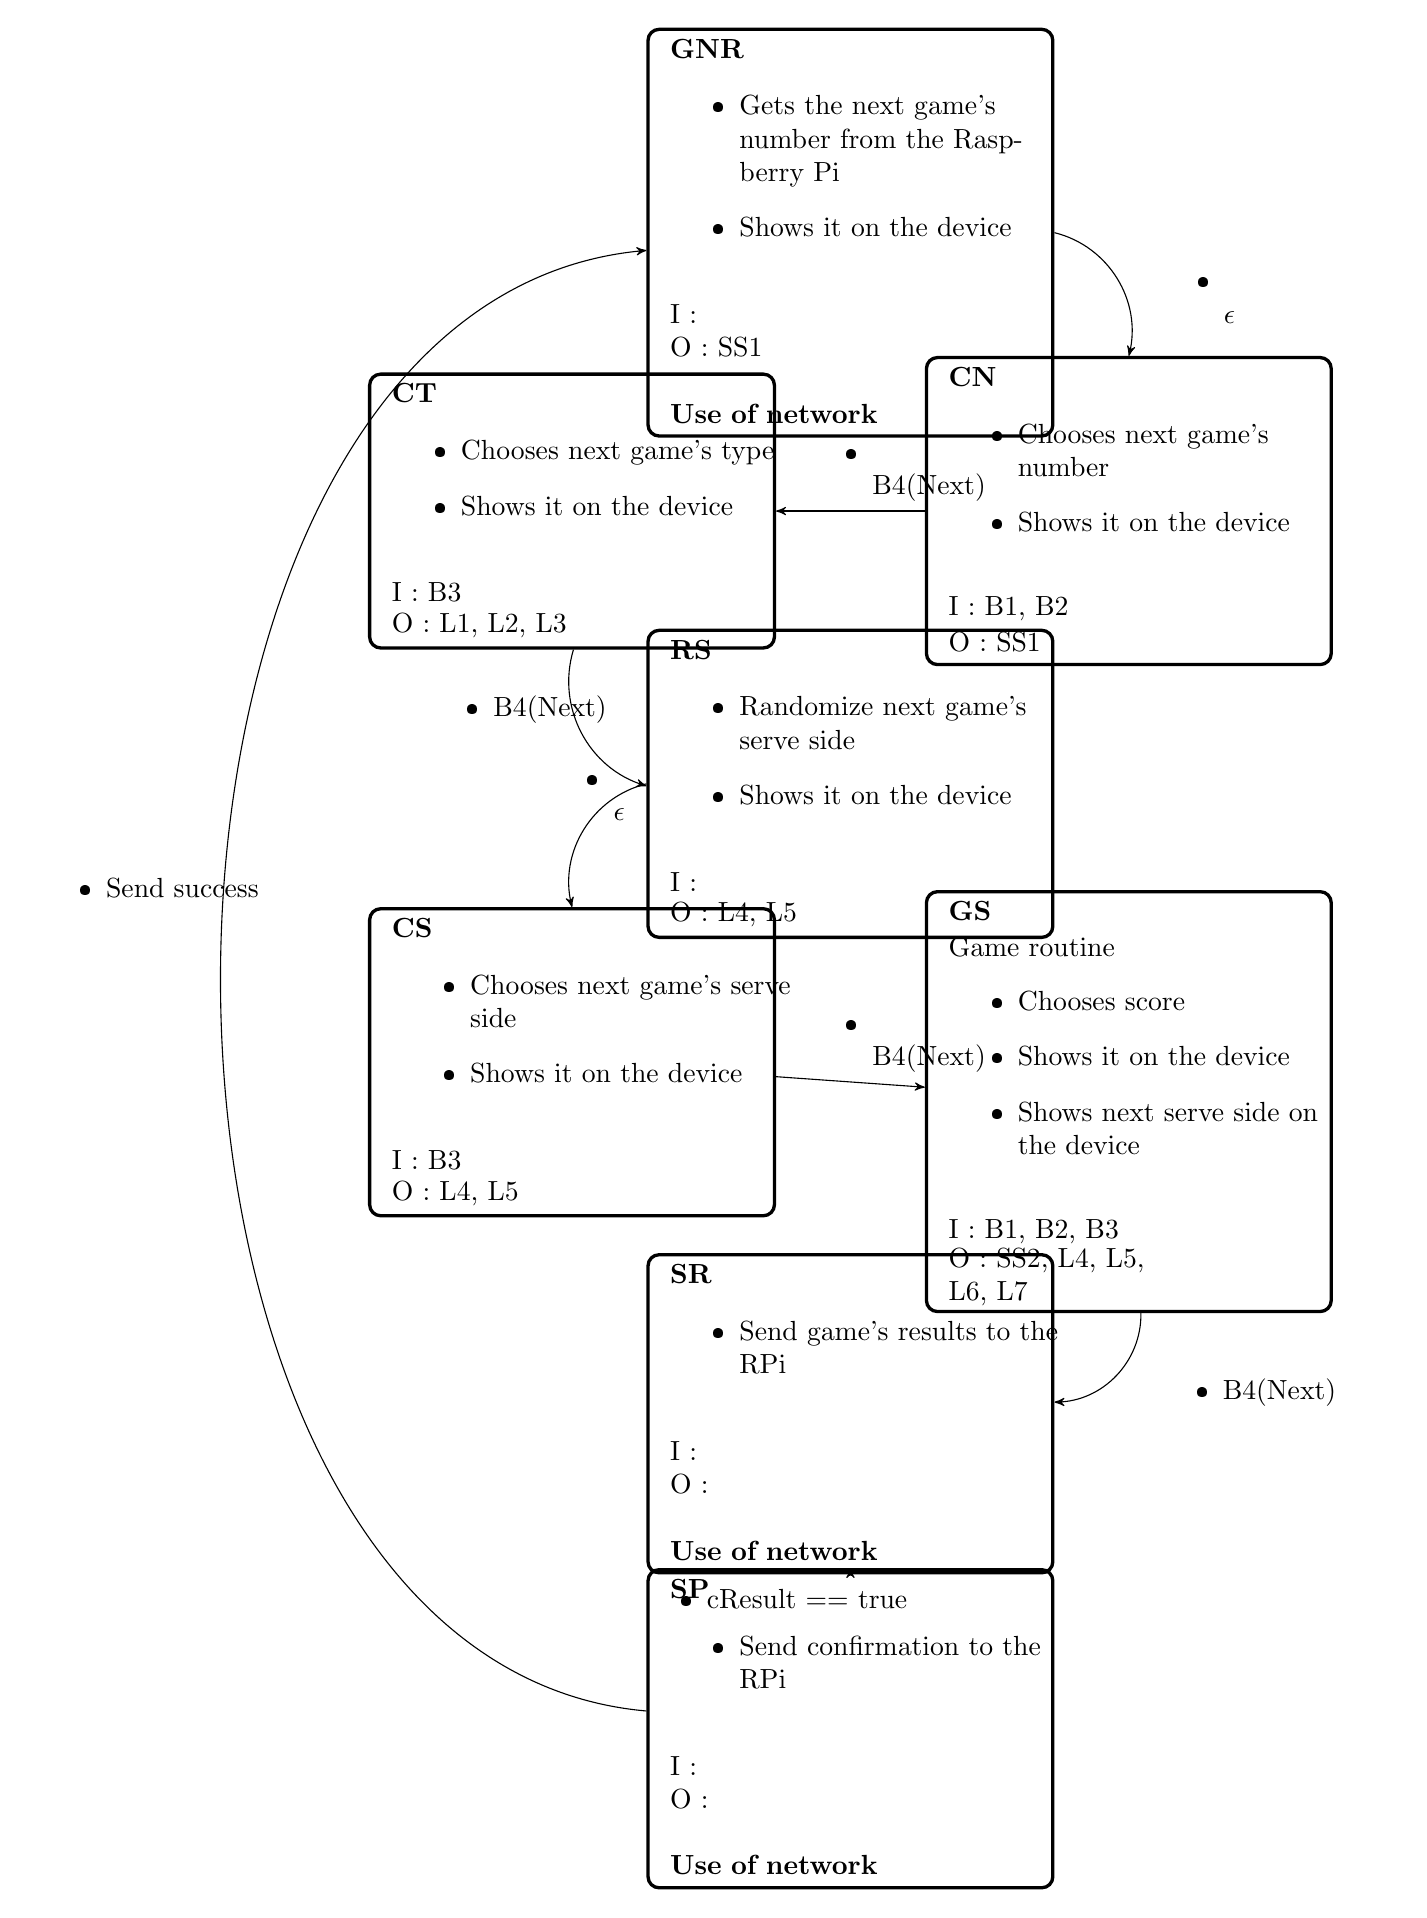
\begin{tikzpicture}[->,>=stealth']
   \node[state,
 node distance=5cm,
 text width=5cm] (GNR) 
 {%
 \begin{tabular}{l}
  \textbf{GNR}\\
  \parbox{5cm}{
  \begin{itemize}
   \item Gets the next game's number from the Raspberry Pi
   \item Shows it on the device 
  \end{itemize}}\\ \\
  \parbox{3cm}{I : }\\ 
  \parbox{3cm}{O : SS1}\\ \\
  \parbox{3cm}{\mbox{\textbf{Use of network}}}
 \end{tabular}
 };
  \node[state,
 below right of=GNR,
 node distance=5cm,
 text width=5cm] (CN) 
 {%
 \begin{tabular}{l}
  \textbf{CN}\\
  \parbox{5cm}{
  \begin{itemize}
   \item Chooses next game's number
   \item Shows it on the device 
  \end{itemize}}\\ \\
  \parbox{3cm}{I : B1, B2}\\ 
  \parbox{3cm}{O : SS1}
 \end{tabular}
 };
  \node[state,
 below left of=GNR,
 node distance=5cm,
 text width=5cm] (CT) 
 {%
 \begin{tabular}{l}
  \textbf{CT}\\
   \parbox{5cm}{
  \begin{itemize}
   \item Chooses next game's type
   \item Shows it on the device 
  \end{itemize}}\\ \\
  \parbox{3cm}{I : B3}\\ 
  \parbox{3cm}{O : L1, L2, L3}
 \end{tabular}
 };

  \node[state,
 below of=GNR,
 node distance=7cm,
 text width=5cm] (RS) 
 {%
 \begin{tabular}{l}
  \textbf{RS}\\
   \parbox{5cm}{
  \begin{itemize}
   \item Randomize next game's serve side
   \item Shows it on the device 
  \end{itemize}}\\ \\
  \parbox{3cm}{I : }\\
  \parbox{3cm}{O : L4, L5}
 \end{tabular}
 };

  \node[state,
 below of=CT,
 node distance=7cm,
 text width=5cm] (CS) 
 {%
 \begin{tabular}{l}
  \textbf{CS}\\
  \ \parbox{5cm}{
  \begin{itemize}
   \item Chooses next game's serve side
   \item Shows it on the device 
  \end{itemize}}\\ \\
  \parbox{3cm}{I : B3}\\ 
  \parbox{3cm}{O : L4, L5}
 \end{tabular}
 };
  \node[state,
 below of=CN,
 node distance=7.5cm,
 text width=5cm] (GS) 
 {%
 \begin{tabular}{l}
  \textbf{GS}\\
  \parbox{5cm}{Game routine}\\
   \parbox{5cm}{
  \begin{itemize}
   \item Chooses score
   \item Shows it on the device
   \item Shows next serve side on the device 
  \end{itemize}}\\ \\
  \parbox{3cm}{I : B1, B2, B3}\\ 
  \parbox{3cm}{O : SS2, L4, L5, L6, L7}
 \end{tabular}
 };
  \node[state,
 below of=RS,
 node distance=8cm,
 text width=5cm] (SR) 
 {%
 \begin{tabular}{l}
  \textbf{SR}\\
   \parbox{5cm}{
  \begin{itemize}
   \item Send game's results to the RPi 
  \end{itemize}}\\ \\
  \parbox{3cm}{I : }\\ 
  \parbox{3cm}{O :}\\ \\
  \parbox{3cm}{\mbox{\textbf{Use of network}}}
 \end{tabular}
 };
  \node[state,
 below of=SR,
 node distance=4cm,
 text width=5cm] (SP) 
 {%
 \begin{tabular}{l}
  \textbf{SP}\\
   \parbox{5cm}{
  \begin{itemize}
   \item Send confirmation to the RPi
  \end{itemize}}\\ \\
  \parbox{3cm}{I : }\\ 
  \parbox{3cm}{O : }\\ \\
  \parbox{3cm}{\mbox{\textbf{Use of network}}}
 \end{tabular}
 };
 % draw the paths and and print some Text below/above the graph
\path 
  (GNR) edge[bend left=45] 
    node[anchor=south,right,text width=1cm,xshift=1em]
    {
      \begin{itemize}
        \item $\epsilon$
      \end{itemize}
    } 
    (CN)
  (CN) edge  
    node[anchor=south,above,text width=1.2cm]
    {
      \begin{itemize}
        \item B4(Next)
      \end{itemize}
    } 
    (CT)
  (CT) edge[bend right=45] 
    node[anchor=south,above,text width=4cm]
    {
      \begin{itemize}
        \item B4(Next)
      \end{itemize}
    } 
    (RS)
  (RS) edge[bend right=45]  
    node[anchor=south,above,text width=1cm]
    {
      \begin{itemize}
        \item $\epsilon$
      \end{itemize}
    } 
    (CS)
  (CS) edge
    node[anchor=south,above,text width=1.2cm]
    {
      \begin{itemize}
        \item B4(Next)
      \end{itemize}
    }                    
    (GS)
  (GS)  edge[bend left=45]
    node[anchor=east,right,text width=3cm,xshift=1em]
    {
      \begin{itemize}
        \item B4(Next)
      \end{itemize}
    } 
    (SR)
  (SR)  edge
    node[anchor=north,below,text width=4cm,yshift=1em,xshift=-2em]
    {
      \begin{itemize}
        \item cResult == true
      \end{itemize}
    } 
    (SP)
  (SP)  edge[bend left=85] 
    node[anchor=west,right,text width=4cm,yshift=4em,xshift=-7em]
    {
      \begin{itemize}
        \item Send success
      \end{itemize}
    } 
    (GNR)
 ;
\end{tikzpicture}
\newpage
% GNR GRAPH
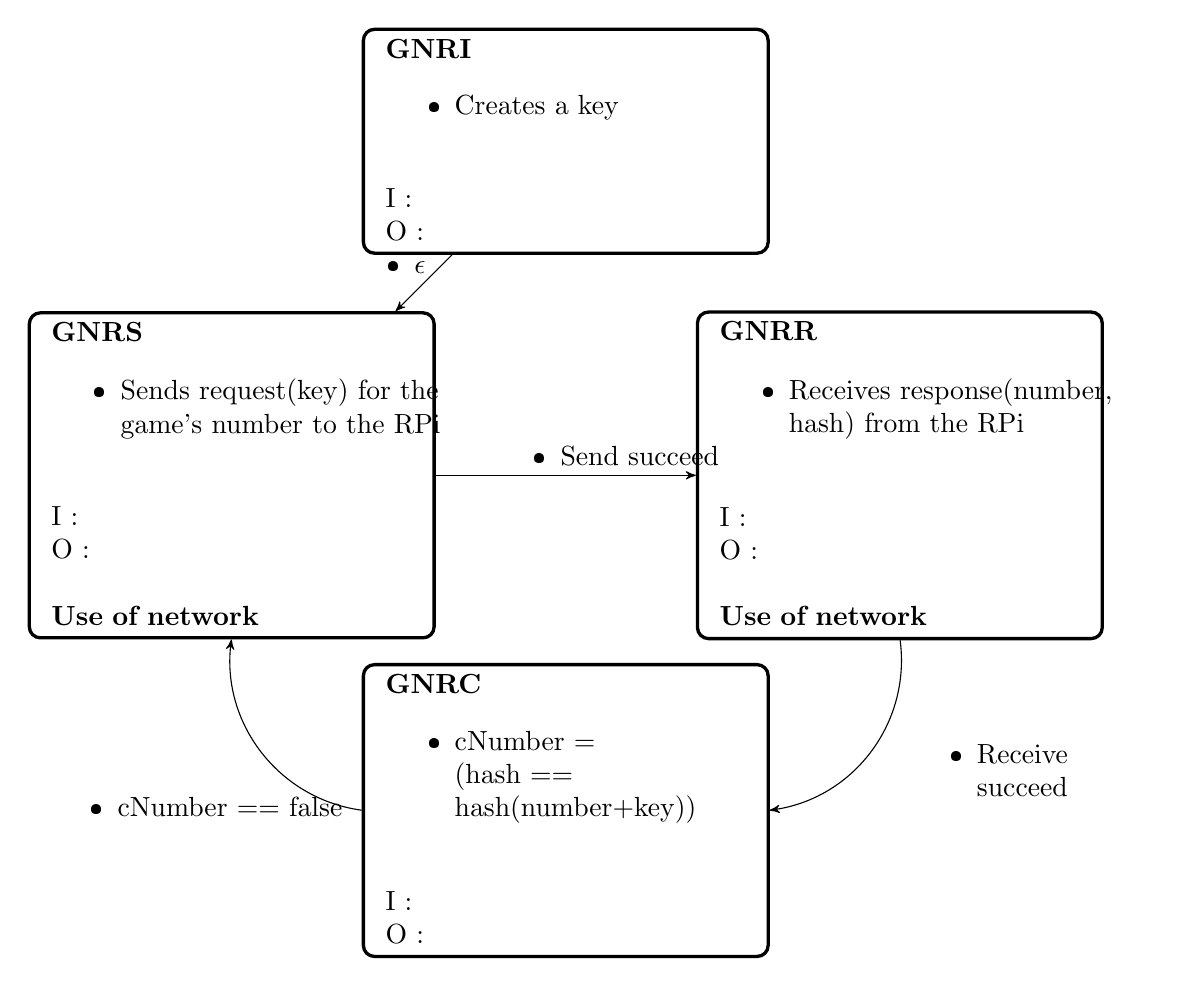
\begin{tikzpicture}[->,>=stealth']
 \node[state, 
 distance=5cm,
 text width=5cm] (GNRI) 
 {%
 \begin{tabular}{l}
  \textbf{GNRI}\\
   \parbox{5cm}{
  \begin{itemize}
   \item Creates a key
  \end{itemize}}\\ \\
  \parbox{3cm}{I : }\\
  \parbox{3cm}{O : }
 \end{tabular}
 };
  \node[state,
 below right of=GNRI,
 node distance=6cm,
 text width=5cm] (GNRR) 
 {%
 \begin{tabular}{l}
  \textbf{GNRR}\\
    \parbox{5cm}{
  \begin{itemize}
   \item Receives response(number, hash) from the RPi 
  \end{itemize}}\\ \\
  \parbox{3cm}{I : }\\
  \parbox{3cm}{O : }\\ \\
  \parbox{3cm}{\mbox{\textbf{Use of network}}}
 \end{tabular}
 };
  \node[state,
 below left of=GNRI,
 node distance=6cm,
 text width=5cm] (GNRS) 
 {%
 \begin{tabular}{l}
  \textbf{GNRS}\\
  \parbox{5cm}{
  \begin{itemize}
   \item Sends request(key) for the game's number to the RPi
  \end{itemize}}\\ \\
  \parbox{3cm}{I : }\\
  \parbox{3cm}{O : }\\ \\
  \parbox{3cm}{\mbox{\textbf{Use of network}}}
 \end{tabular}
 };
   \node[state,
 below of=GNRI,
 node distance=8.5cm,
 text width=5cm] (GNRC) 
 {%
 \begin{tabular}{l}
  \textbf{GNRC}\\
   \parbox{5cm}{
  \begin{itemize}
   \item cNumber = \\(hash == hash(number+key))
  \end{itemize}}\\ \\
  \parbox{3cm}{I : }\\
  \parbox{3cm}{O : }
 \end{tabular}
 };
  \path 
  (GNRI) edge  
    node[anchor=south,above,text width=2cm]
    {
      \begin{itemize}
        \item $\epsilon$
      \end{itemize}
    } 
    (GNRS)
  (GNRS) edge
    node[above,text width=4cm,xshift=3em]
    {
      \begin{itemize}
        \item Send succeed
      \end{itemize}
    }                    
    (GNRR)
  (GNRR)  edge[bend left=45]
    node[anchor=east,right,text width=3cm,xshift=1em]
    {
      \begin{itemize}
        \item Receive succeed
      \end{itemize}
    } 
    (GNRC)

  (GNRC)  edge[bend left=45] 
    node[anchor=north,below,text width=4cm,xshift=-2em]
    {
      \begin{itemize}
        \item cNumber == false
      \end{itemize}
    } 
    (GNRS)
 ;
\end{tikzpicture}

% SR GRAPH
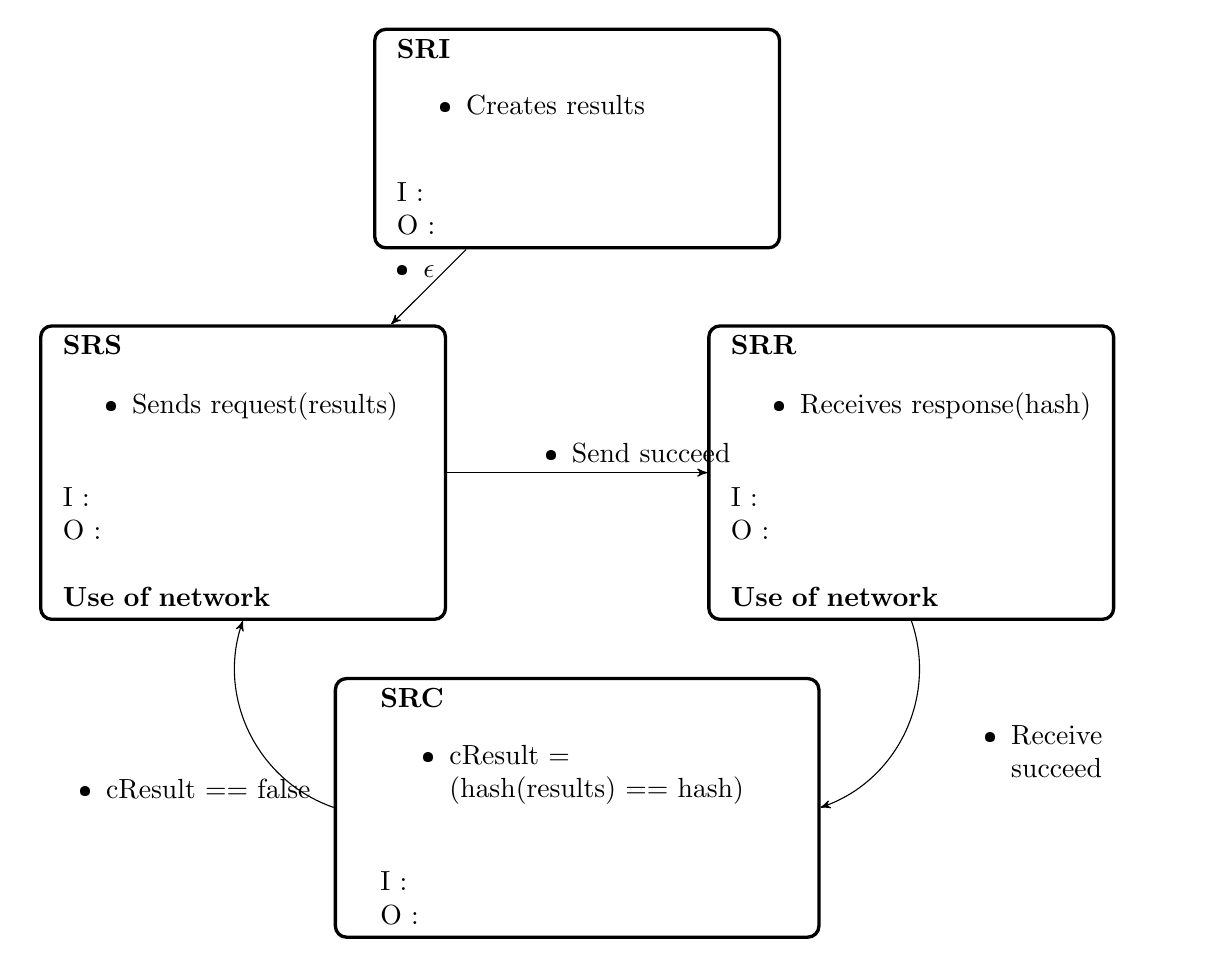
\begin{tikzpicture}[->,>=stealth']
  \node[state,
 node distance=0cm,
 text width=5cm] (SRI) 
 {%
 \begin{tabular}{l}
  \textbf{SRI}\\
   \parbox{5cm}{
  \begin{itemize}
   \item Creates results
  \end{itemize}}\\ \\
  \parbox{3cm}{I : }\\
  \parbox{3cm}{O :}
 \end{tabular}
 };
  \node[state,
 below left of=SRI,
 node distance=6cm,
 text width=5cm] (SRS) 
 {%
 \begin{tabular}{l}
  \textbf{SRS}\\
   \parbox{5cm}{
  \begin{itemize}
   \item Sends request(results)
  \end{itemize}}\\ \\
  \parbox{3cm}{I : }\\ 
  \parbox{3cm}{O : }\\ \\
  \parbox{3cm}{\mbox{\textbf{Use of network}}}
 \end{tabular}
 };
  \node[state,
 below right of=SRI,
 node distance=6cm,
 text width=5cm] (SRR) 
 {%
 \begin{tabular}{l}
  \textbf{SRR}\\
   \parbox{5cm}{
  \begin{itemize}
   \item Receives response(hash)
  \end{itemize}}\\ \\
  \parbox{3cm}{I : }\\
  \parbox{3cm}{O :}\\ \\
  \parbox{3cm}{\mbox{\textbf{Use of network}}}
 \end{tabular}
 };
  \node[state,
 below of=SRI,
 node distance=8.5cm,
 text width=6cm] (SRC) 
 {%
 \begin{tabular}{l}
  \textbf{SRC}\\
   \parbox{5cm}{
  \begin{itemize}
   \item cResult = \\(hash(results) == hash)
  \end{itemize}}\\ \\
  \parbox{3cm}{I :}\\
  \parbox{3cm}{O :}
 \end{tabular}
 };
\path 
  (SRI) edge  
    node[anchor=south,above,text width=4cm,xshift=3em]
    {
      \begin{itemize}
        \item $\epsilon$
      \end{itemize}
    }           
    (SRS)
  (SRS) edge
    node[anchor=south,above,text width=4cm,xshift=3em]
    {
      \begin{itemize}
        \item Send succeed
      \end{itemize}
    }                    
    (SRR)
  (SRR)  edge[bend left=45]
    node[anchor=east,right,text width=3cm,xshift=1em]
    {
      \begin{itemize}
        \item Receive succeed
      \end{itemize}
    } 
    (SRC)

  (SRC)  edge[bend left=45] 
    node[anchor=north,below,text width=4cm,xshift=-2em]
    {
      \begin{itemize}
        \item cResult == false
      \end{itemize}
    } 
    (SRS)
 ;
\end{tikzpicture}
\end{document}